\documentclass[11pt]{article}

\usepackage[T2A]{fontenc}
\usepackage[utf8]{inputenc}
\usepackage[russian]{babel}

\usepackage{hyphenat}
\hyphenation{ма-те-ма-ти-ка вос-ста-нав-ли-вать}

\usepackage[a4paper,margin=2cm]{geometry}

\usepackage{graphicx}
\usepackage[intlimits]{amsmath}
\usepackage{amssymb}
\usepackage{amsmath}
\usepackage{subcaption}
\usepackage{wrapfig}
\usepackage{float}
\usepackage{fancyhdr}
\usepackage{mathtools}
\usepackage{tensor}
\usepackage{pgf}
\usepackage[parfill]{parskip}
\usepackage{array}
\usepackage[utf8]{inputenc}\DeclareUnicodeCharacter{2212}{-}

\newcommand{\rot}[1]{[\nabla, \mathbf{#1}]}
\newcommand{\di}[1]{(\nabla, \mathbf{#1})}
\newcommand{\ve}[1]{\mathbf{#1}}
\newcommand{\re}[1]{(\ref{#1})}


\begin{document}
  \title{Работа 5.1.3. Эффект Рамзауэра}
  \author{Фролов Александр}
  \date{}
  \maketitle
  
  \paragraph{Цель работы:}исследовать энергетическую зависимость веротности рассеяния электронов атомами ксенона, определить энергии электронов, при которых наблюдается просветление ксенона и оценить размер его внешней электронной оболочки. \\
  \par
     \begin{figure}[H]
\centering
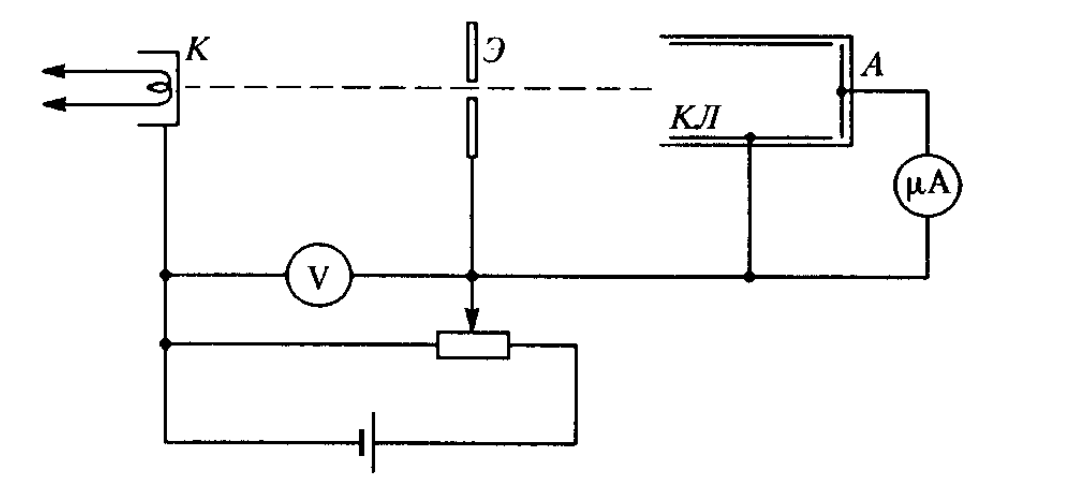
\includegraphics[width=0.95\linewidth]{ramz.png}
\caption{Схема эксперимента Рамзауэра}
\end{figure}
  Рассмотрим схему опыта Рамзауэра, приведенную на рис. 1. Пучое электронов, вылетая из накаленного катода К, проходит ускоряющую разность потенциалов V, приложенную между катодом и электродом Э, и приобретает энергию $E = mv^2/2 = eV$. При прохождени через газ часть электронов рассеивается на атомах и собирается где-то в стороне коллектором КЛ, а часть проходит дальше и попадает на анод А, создавая анодный ток I. Этот ток пропорционален числу прошедших электронов и потому непосредственно характеризует проницаемость газа для электронного пучка в зависимости от ускоряющего напряжения. То есть с ростом $V$ можно ожидать монотонное возрастание тока.
  \\
  Но этого не происходит. Рассмотрим процесс с точки зрения квантовой теории. Внутри атома потенциальная энергия налетающего электрона $U$ отлична от нуля, и его скорость изменяется в соответствии с законом сохранения:
  \[
   E = \frac{mv^2}{2} = \frac{mv'^2}{2} + U.
  \]
  Но это значит и что меняется длина его волны де Бройля. То есть атом ведет себя как преломляющая среда. \\
  Будем считать, что атом рассеивается на прямоугольной потенциальной яме конечной шириной $l$ и глубиной $U_0$. Уравнение Шредингера в данном случае:
  \[
   \psi'' + k^2\psi = 0,
  \]
  \[
   k^2 = \begin{dcases} 
   k_1^2 = 2mE/\hslash^2, \text{  в I и III} \\
   k_2^2 = 2m(E + U_0)/\hslash^2, \text{ в II}
   \end{dcases}
  \]
  Коэффициент прохождения определяется как:
  \[
   D = \frac{16 k_1^2 k_2^2}{16k_1^2k_2^2 + 4(k_1^2 - k_2^2)^2\sin^2(k_2l)}
  \]
  Этот коэффициент имеет ряд чередующихся максимумов и минимумов. Он максимален при условии:
  \[
   k_2l = \sqrt{\frac{2m(E + U)}{\hslash^2}}l, \hspace{0.5cm} l =\pi n, \hspace{0.5cm} n=1,2,3.
  \]
    \begin{figure}[H]
\centering{
 \begin{subfigure}[b]{0.45\textwidth}
        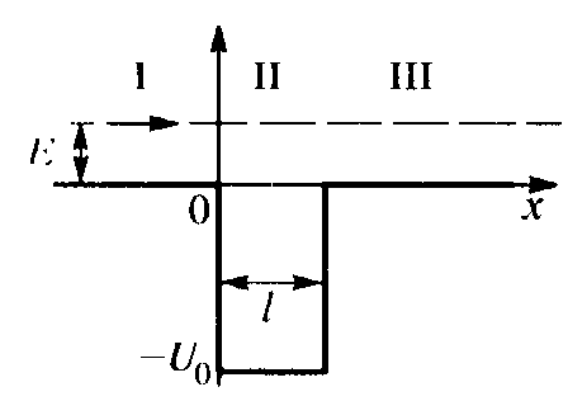
\includegraphics[width=\textwidth]{ya.png}
        \caption{Потенциальная яма атома}
    \end{subfigure}
    \begin{subfigure}[b]{0.45\textwidth}
        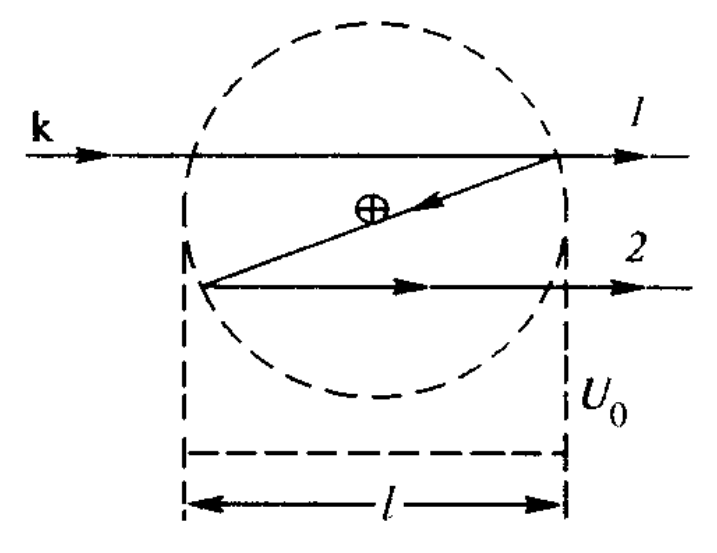
\includegraphics[width=\textwidth]{int.png}
        \caption{Интерференция волн де Бройля в атоме}
    \end{subfigure}
}

\end{figure}
  Можно также рассмотреть интерференцию волн де Бройля в атоме. Движущемуся электрону соответсвует волна де Бройля длины $\lambda = h/mv$. Если его кинетическая энергия мала, то $E = mv^2/2$ и $\lambda = h/\sqrt{2mE}$. При двжении через атом длина волны становится меньше и равна $\lambda_1 = h/\sqrt{2m(E + U_0)}$, где $U_0$ --- глубина атомного потенциала. При этом волна отражается от границ атомного потенциала, и происходит интерференция прошедшей и отраженной волн(они когерентны). Если геометрическая разность хода между этими волнами равна $\Delta = 2l = \lambda_1$, то прошедшая волна усилится отраженной, что даст первый интерференционный максимум:
  \begin{equation} \label{max}
   2l = \frac{h}{\sqrt{2m(E_1 + U_0)}}.
  \end{equation}
  Прошедшая волна ослабится, если $\Delta = 2l = (3/2)\lambda_1$, т.е условие первого интерференционного минимума запишется как 
  \begin{equation} \label{min}
   2l = \frac{3}{2}\frac{h}{\sqrt{2m(E_2 + U_0)}}.
  \end{equation}
  Исключив $U_0$, можно найти эффективный размер атома $l$:
  \begin{equation} \label{l}
   l = \frac{h\sqrt{5}}{\sqrt{32m(E_2 - E_1)}}.
  \end{equation}
  Также можно рассчитать глубину потенциальной ямы:
  \begin{equation} \label{u0}
   U_0 = \frac{4}{5}E_2 - \frac{9}{5}E_1.
  \end{equation}
  \subsubsection*{Экспериментальная установка}
  Рассмотрим вольт-амперную характеристику тиратрона. Выделим в газе на расстоянии $x$ тонкий слой длины $dx$ c площадью поперечного сечения $S$. В этом слое сожержится $\nu = n_a S dx$ атомов газа. Суммарная рассеивающая поверхность этих атомов $\Delta = \Delta_a \nu$, $\Delta_a$ --- площадь поперечного сечения атома. $dN$ --- убыль потока электронов посл прохождения этого слоя; тогда $dN/N(x)$ --- вероятность рассеяния в этом слое. Эта вероятность равна произведению двух событий: первое --- то, что электрон встретил атом газа, и второе --- электрон на нем рассеялся:
  \[
   -\frac{dN}{N(x)} = \frac{\Delta}{S}w(V) = n_a\Delta_aw(V)dx.
  \]
  Остюда уравнение ВАХ:
  \[
   I_a = I_0 e^{-Cw(v)}, \hspace{0.5cm} C = Ln_a\Delta_a,
  \]
  где $I_0$ --- ток катода, $I_a$ --- анодный ток. \\
  Отсюда по измеренной ВАХ:
  \begin{equation} \label{w}
   w(V) = -\frac{1}{C}\ln\frac{I_a(V)}{I_0}.
  \end{equation}
  \begin{figure}[H]
\centering{
 \begin{subfigure}[b]{0.3\textwidth}
        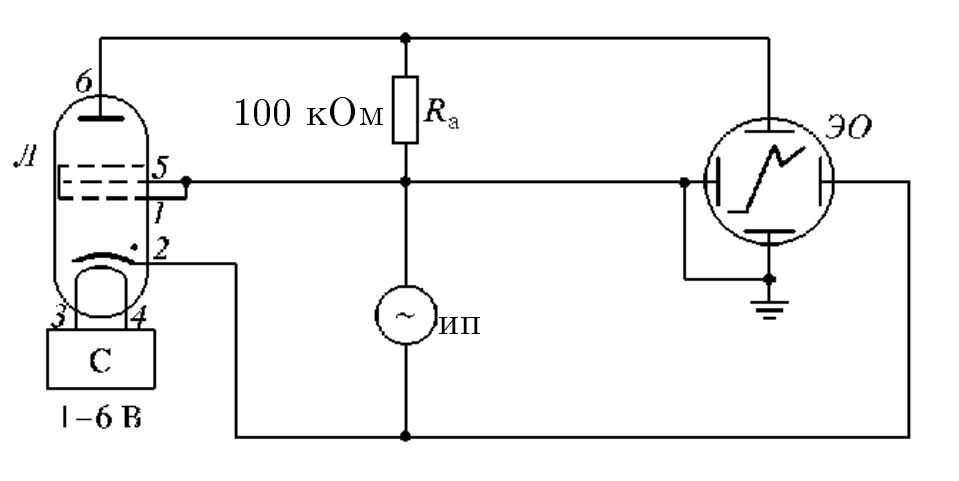
\includegraphics[width=\textwidth]{sch.png}
        \caption{}
    \end{subfigure}
    \begin{subfigure}[b]{0.6\textwidth}
        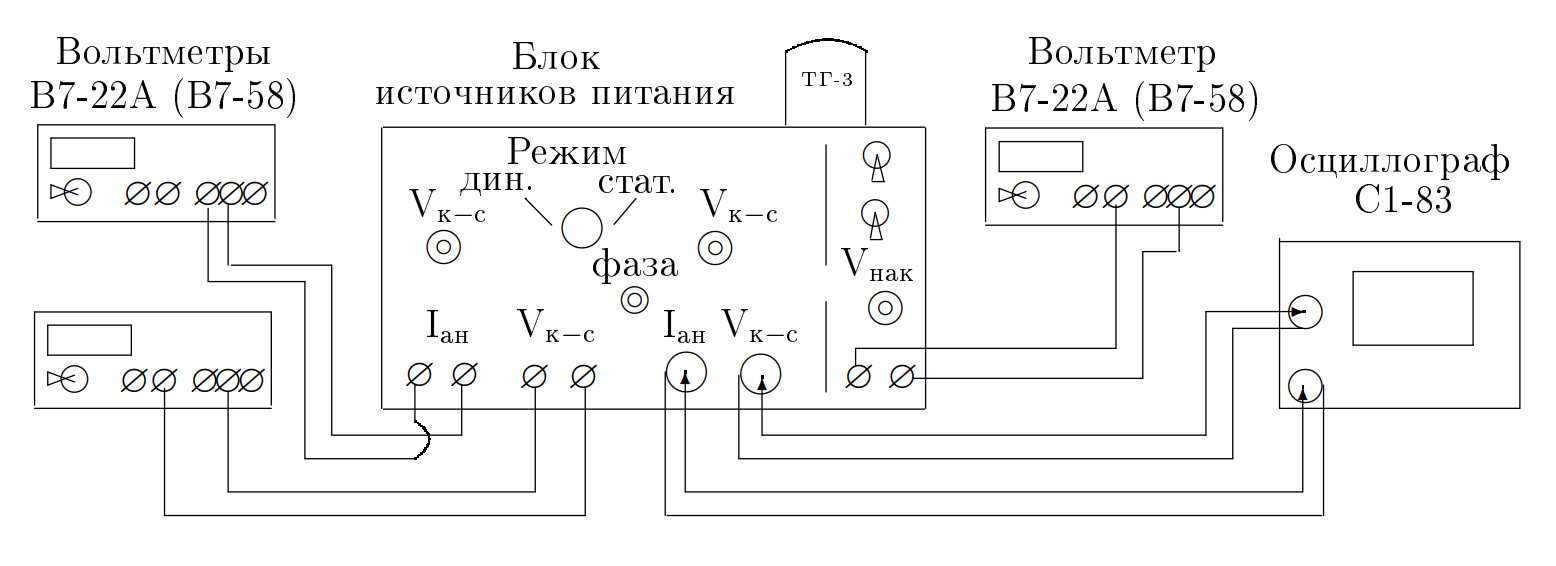
\includegraphics[width=\textwidth]{sch2.png}
        \caption{}
    \end{subfigure}
}
\caption{Схема подключения тиратрона (а) и блок-схема установки (b).}
\end{figure}
  \subsubsection*{Ход работы}
  Проведем исследования в динамическом режиме. \\
  \begin{figure}[H]
\centering{
 \begin{subfigure}[b]{0.45\textwidth}
        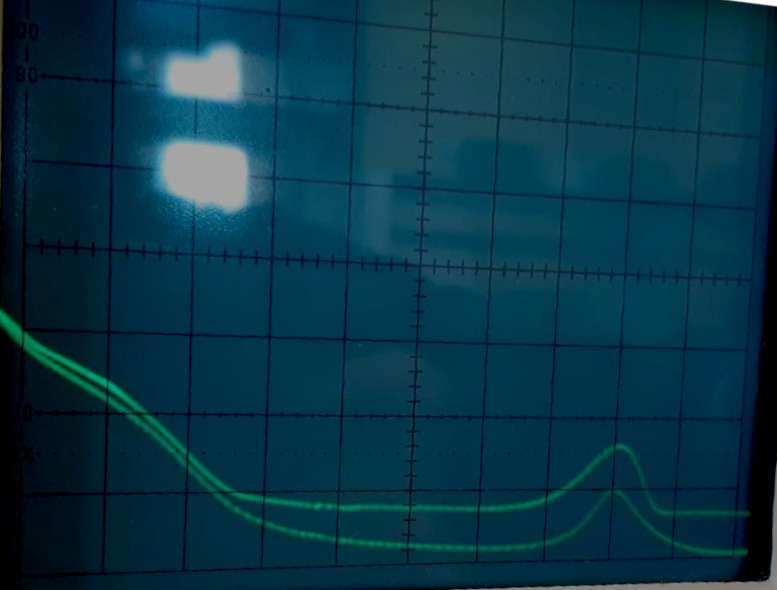
\includegraphics[width=\textwidth]{23.jpg}
        \caption{2.3 В}
    \end{subfigure}
    \begin{subfigure}[b]{0.45\textwidth}
        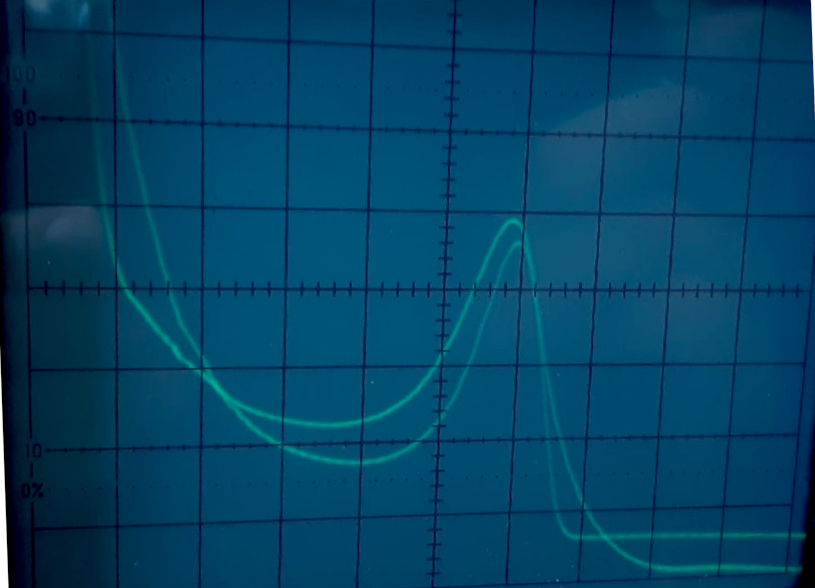
\includegraphics[width=\textwidth]{29.jpg}
        \caption{2.9 В}
    \end{subfigure}
}
\end{figure}
Для напряжения накала равного 2.3 В:
$E_1 = 1.6 \pm 0.2$ \\
$E_2 = 6 \pm 0.2$ \\
Отсюда посчитаем(приняв $U_0$ = 2.5) тремя способами размер электронной оболочки атома: \\
$l_1 = 3.3 \pm 0.4 $ \AA{} \\
$l_2 = 3.0 \pm 0.4$ \AA{} \\
$l_3 = 3.2 \pm 0.4$ \AA{} \\
Тогда $\bar{l} = 3.2 \pm 0.1$ \AA{}. \\
Оценим глубину ямы: $U_0 = 1.9 \pm 0.2$ эВ. \\
Теперь то же для напряжения накала в 2.9 В: \\
$E_1 = 2 \pm 0.2$ \\
$E_2 = 6 \pm 0.2$ \\
Отсюда посчитаем(приняв $U_0$ = 2.5) тремя способами размер электронной оболочки атома: \\
$l_1 = 3.4 \pm 0.4 $ \AA{} \\
$l_2 = 2.9 \pm 0.3$ \AA{} \\
$l_3 = 3.2 \pm 0.2$ \AA{} \\
Тогда $\bar{l} = 3.2 \pm 0.2$ \AA{}. \\
Оценим глубину ямы: $U_0 = 1.9 \pm 0.2$ эВ. \\
Также отметим, что напряжение резко возрастает примерно при 12 В, из чего можно заключить, что тиратрон наполнен ксеноном --- его потенциал ионизации равен 12.1 В. \\
  Вольт-амперная характеристика тиратрона, полученная измерением в статическом режиме:
   \begin{figure}[H]
\centering
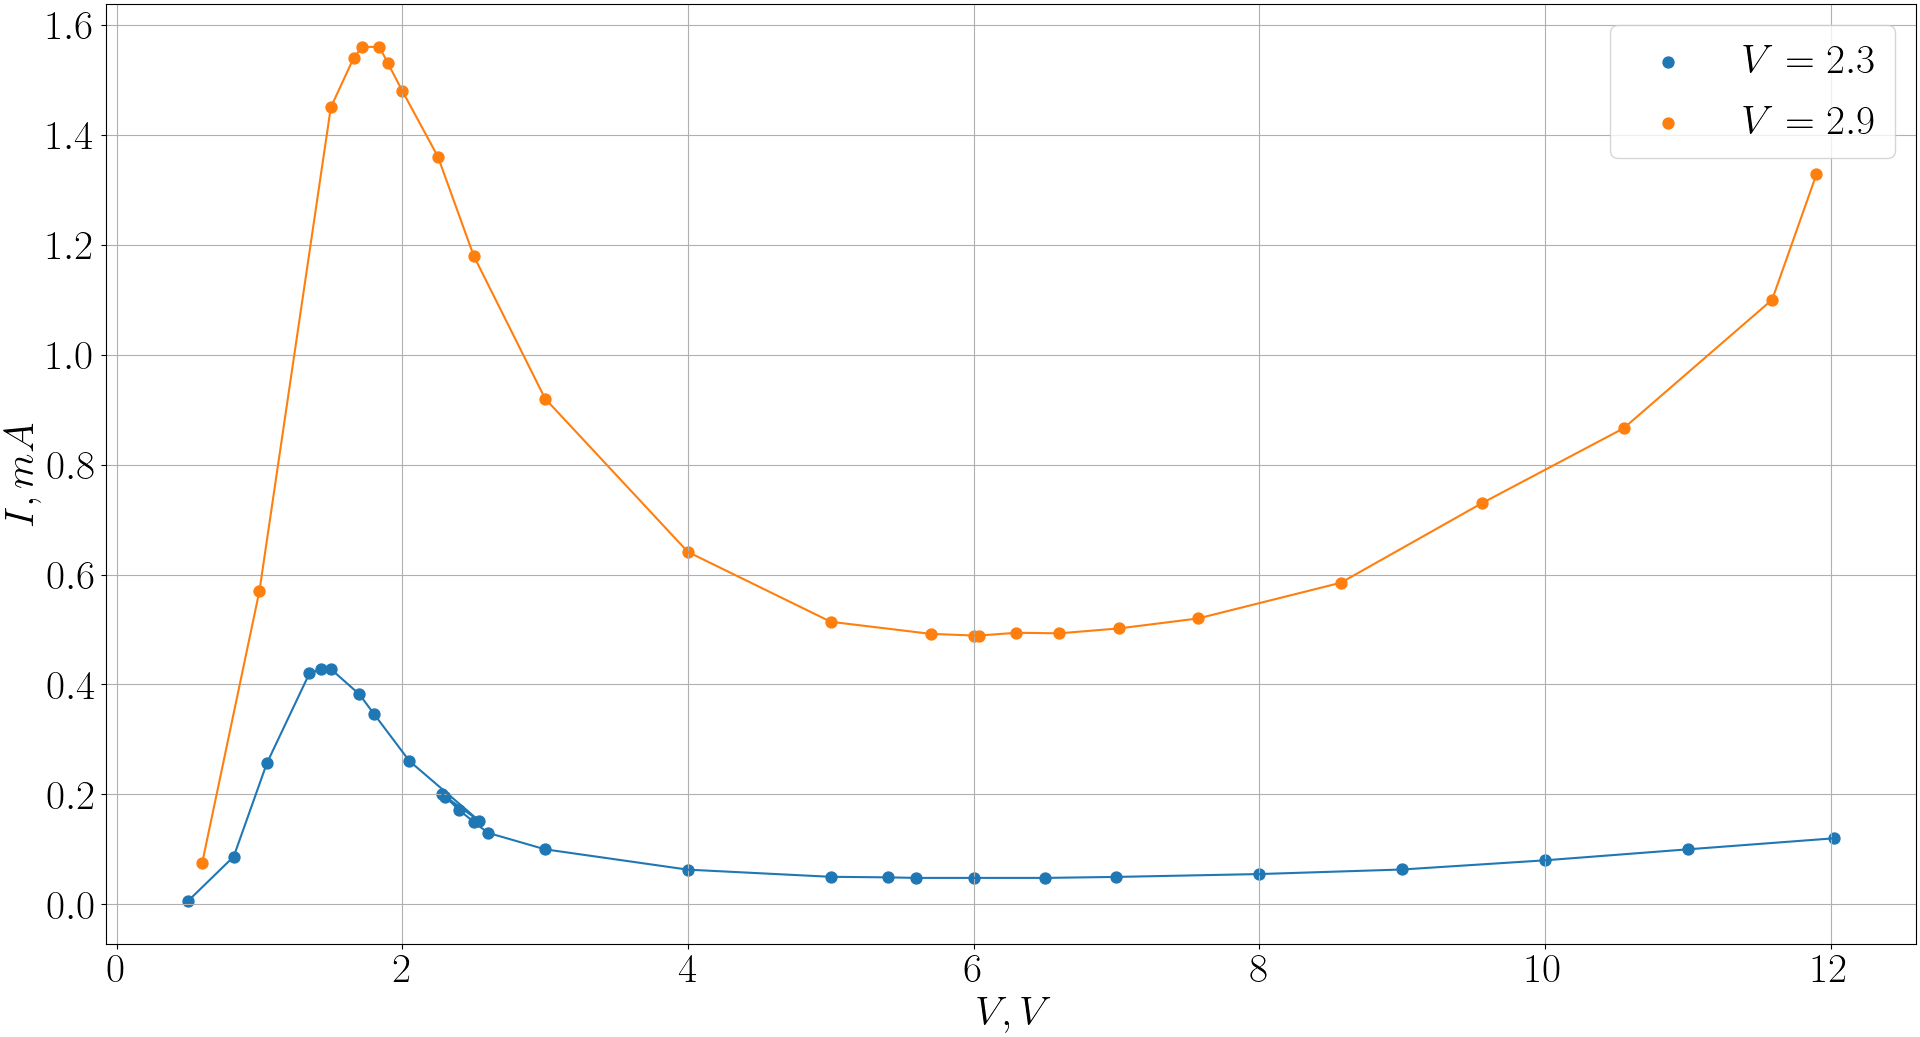
\includegraphics[width=0.95\linewidth]{f1.png}
\caption{Зависимость анодного тока от энергии электронов}
\end{figure}
Повторим вычисления эффективного размера атома и глубины его потенциальной ямы: \\
$V_\text{н} = 2.3$: \\
$E_1 = 1.5 \pm 0.2$ \\
$E_2 = 6 \pm 0.2$ \\
Отсюда посчитаем(приняв $U_0$ = 2.5) тремя способами размер электронной оболочки атома: \\
$l_1 = 3.2 \pm 0.4 $ \AA{} \\
$l_2 = 3.1 \pm 0.4$ \AA{} \\
$l_3 = 3.2 \pm 0.3$ \AA{} \\
Тогда $\bar{l} = 3.2 \pm 0.1$ \AA{}. \\
Оценим глубину ямы: $U_0 = 2.1 \pm 0.2$ эВ. \\

$V_\text{н} = 2.9$: \\
$E_1 = 1.8 \pm 0.2$ \\
$E_2 = 6 \pm 0.2$ \\
Отсюда посчитаем(приняв $U_0$ = 2.5) тремя способами размер электронной оболочки атома: \\
$l_1 = 3.3 \pm 0.4 $ \AA{} \\
$l_2 = 2.9 \pm 0.3$ \AA{} \\
$l_3 = 3.2 \pm 0.2$ \AA{} \\
Тогда $\bar{l} = 3.1 \pm 0.2$ \AA{}. \\
Оценим глубину ямы: $U_0 = 1.6 \pm 0.2$ эВ. \\
Построим график зависимости вероятности рассеяния от энергии с точностью до константы:
\begin{figure}[H]
\centering
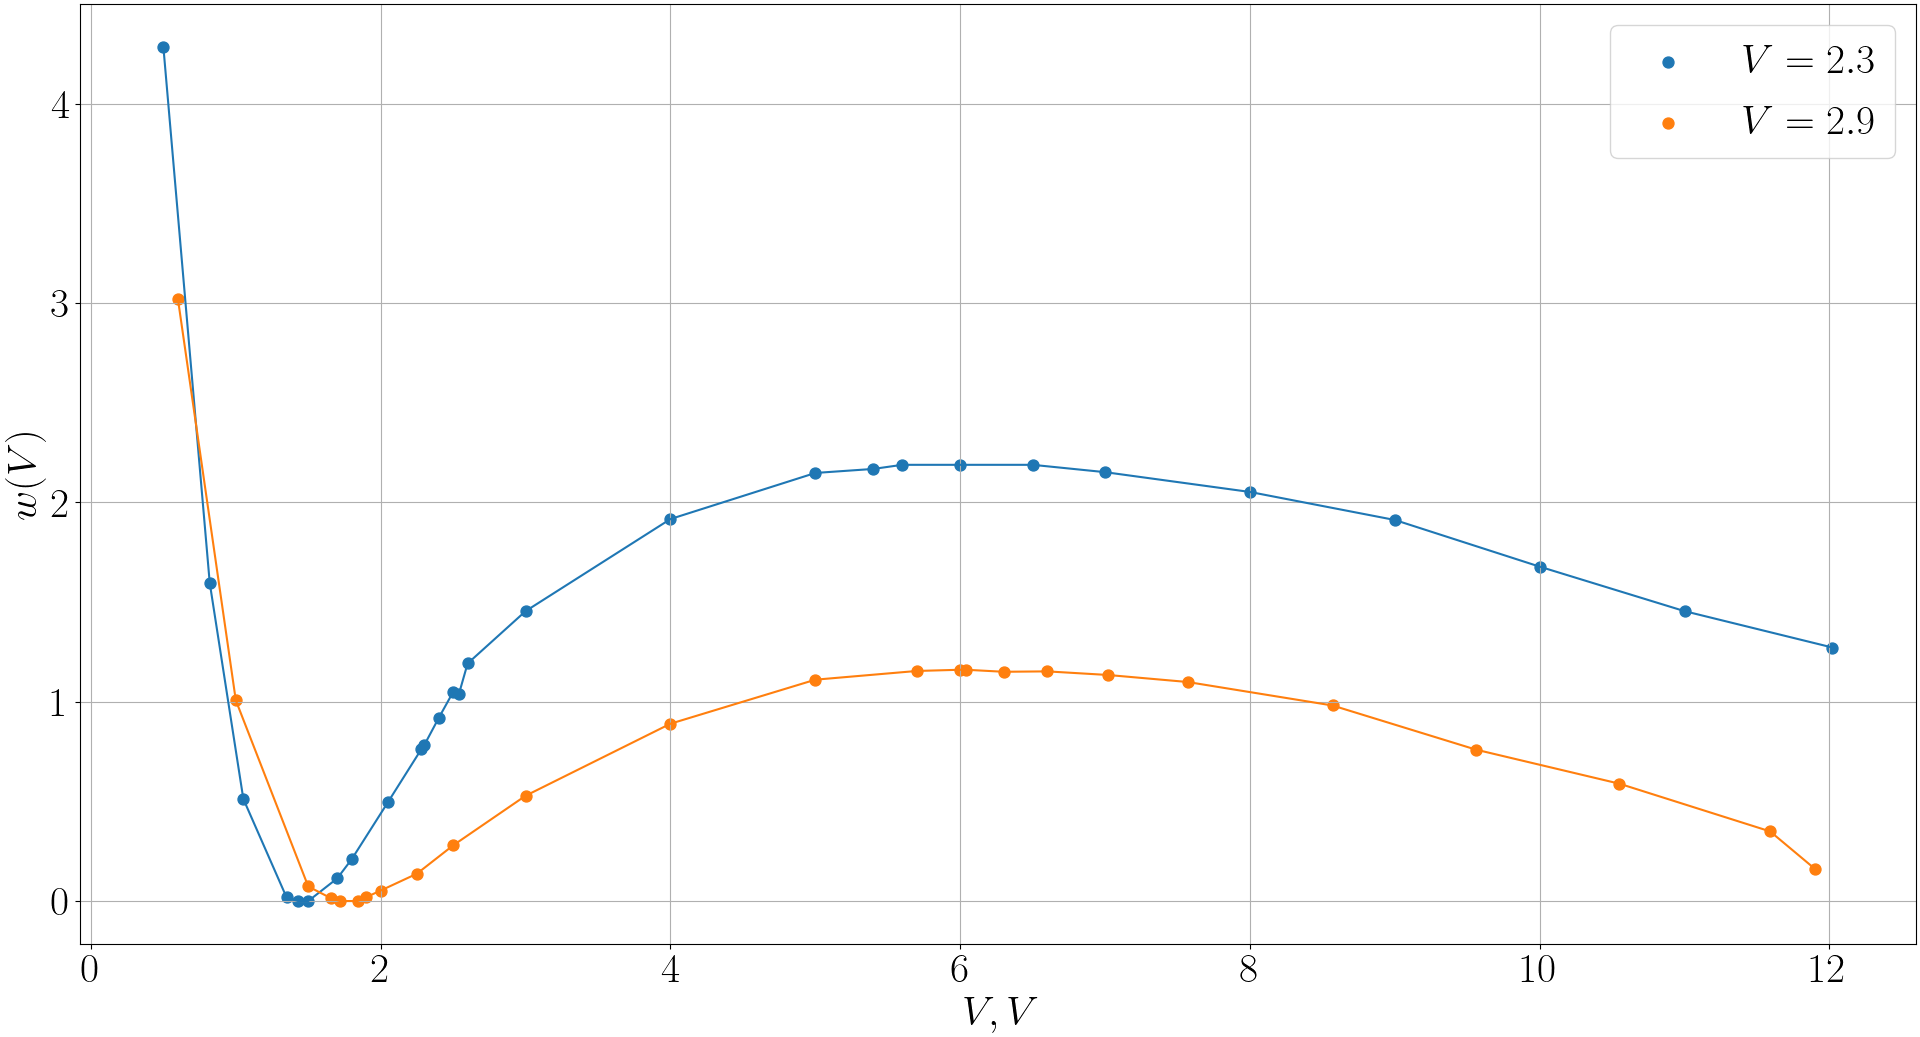
\includegraphics[width=0.95\linewidth]{f2.png}
\caption{Зависимость вероятности рассеяния от энергии}
\end{figure}
Оценим также, при каких напряжениях должны появиться второй и третий максимумы. Для этого преобразуем условие просветления:
\[
 \sqrt{E_n + U_0} \frac{l}{1.95} = \pi n,
\]
где энергии --- в эВ, а $l$ --- в \AA{}. Отсюда можно получить:
\[
 E_n = \left(\frac{1.95\pi}{l}\right)^2(n^2 - 1) + E_1.
\]
Получим, что при напряжении накала в 2.3 В у нас должны были быть максимумы при 12.8 и 31.6 эВ, а при 2.9 --- при 13.1 и 32 эВ соответственно. Так как при таких энергиях уже начинается пробой(да и на приборе дальше ручка не крутится), мы, ожидаемо, не смогли их увидеть.
\subsubsection*{Вывод}
Мы смогли увидеть эффект Рамзауэра при рассеянии электронов на атомах ксенона; из полученных данных смогли оценить размеры атомов газа и глубину потенциальной ямы, которой можно их представить. Полученные величины по порядку совпадают с ожидаемыми (размер атома порядка 1 ангстрема; потенциал порядка 1-10 эВ).

\end{document}
